\documentclass[12pt,a4paper]{article}

\usepackage[utf8]{inputenc}
\usepackage[T1]{fontenc}
\usepackage{mathptmx}
\usepackage{geometry}
\usepackage{graphicx}
\usepackage{booktabs}
\usepackage{array}
\usepackage{tabularx}
\usepackage{caption}
\usepackage{subcaption}
\usepackage{tikz}
\usepackage{microtype}
\usepackage[natbibapa]{apacite}
\usepackage{hyperref}
\usetikzlibrary{arrows.meta,positioning,shapes.geometric,calc}
\definecolor{siteblue}{RGB}{0,113,188}
\definecolor{sitegreen}{RGB}{30,145,95}
\definecolor{siteorange}{RGB}{230,126,34}

\geometry{margin=2.5cm}
\captionsetup{font=small,labelfont=bf}
\setlength{\parskip}{0pt}
\setlength{\textfloatsep}{9pt plus 1pt minus 2pt}
\setlength{\floatsep}{7pt plus 1pt minus 2pt}
\setlength{\intextsep}{9pt plus 1pt minus 2pt}
\emergencystretch=2em
\hypersetup{
  colorlinks=true,
  linkcolor=black,
  citecolor=black,
  urlcolor=blue
}

\title{\textbf{A ROS 2 Digital Twin for Construction Robot Inspection}}
\author{
Tian Tan\\
Department of Civil Engineering\\
The University of Hong Kong\\
Hong Kong, China\\
\texttt{tiantan05@connect.hku.hk}
}
\date{}

\begin{document}
\maketitle

\begin{abstract}
Construction inspection still relies on manual site walks, visual judgement, and records that are often separated from the actual work front. Mobile robots can make inspection more repeatable, but construction sites are cluttered, changing, and safety-critical, so autonomy should first be tested in a controlled digital environment. This paper presents a ROS 2-based construction robot digital twin prototype for an indoor inspection task. The system combines Gazebo simulation, a four-wheel mobile robot model, LiDAR and RGB sensing, Nav2 autonomous navigation, SLAM-ready mapping, mission orchestration, and a browser-based FastAPI dashboard. The implemented task is to start from point A, navigate through a site-like room, approach a wall-mounted AprilTag target at point B, and report mission state and telemetry to an operator. The codebase was reviewed at the package and node level to document the implemented architecture rather than only the final demonstration. The prototype connects simulation, navigation, telemetry, and human supervision into an executable construction robot twin. Its limits are also clear: the AprilTag is currently a known map target rather than a detected visual pose, the platform is a mobile inspection robot rather than a mobile manipulator, and the work has not been deployed on physical hardware.
\end{abstract}

\noindent\textbf{Keywords:} construction digital twin; construction robotics; ROS 2; Gazebo; Nav2; mobile robot inspection

\section{Introduction}

Construction projects generate decisions in places where information is incomplete and conditions change quickly. A route that is clear in the morning can become blocked by material stacks in the afternoon. Temporary fences and no-go zones are moved as work fronts progress. Inspection staff need to confirm progress, safety conditions, and asset state, but manual site walks are time-consuming and hard to repeat at high frequency. This is one reason mobile robots are attractive for construction monitoring: they can collect data along planned routes and return structured state information to an operator.

The difficulty is that construction sites are not designed for robots. Floors may be uneven, obstacles are irregular, work zones are shared with people, and the relevant information is not only geometric. A robot must know where it is, where it is allowed to move, what it is trying to inspect, and whether its current behaviour is safe. These requirements make a digital twin more useful than a simple animation. A useful construction robot twin should combine a virtual site, a robot model, sensor streams, navigation logic, mission state, and a decision interface.

This project implements that idea at prototype scale. It contains a ROS 2 workspace with separate packages for robot description, simulation, navigation, mission logic, and a local web dashboard. The robot is a four-wheel mobile inspection platform with LiDAR, camera, odometry, transforms, and a pan/tilt gimbal. The site is a Gazebo room with walls, material-like obstacles, barriers, a tool chest, an inspection column, and a wall-mounted AprilTag. The task is deliberately narrow: the robot starts at point A, navigates to the AprilTag approach point B, and reports the mission as complete.

The work is not presented as a new navigation algorithm. Its value is in the integration: a small but reproducible digital twin architecture for construction robot inspection, with simulation, navigation, mission logic, telemetry, and operator feedback working together. The discussion also keeps the scope explicit. Although the CIVIL 8025 Project 4 direction mentions mobile manipulation and MoveIt 2 as possible elements, this implementation is a mobile inspection robot twin and does not include an arm, MoveIt 2 planning, or real AprilTag pose estimation.

\section{Literature Review}

\subsection{Construction digital twins}

Digital twin research in construction has moved beyond the idea of a 3D model. \citet{boje2020semantic} argue that a semantic construction digital twin should connect model information, data streams, and reasoning so that the digital representation can support decisions. This distinction matters here because a Gazebo model alone would not be enough. The project becomes closer to a twin when the simulated robot state, sensor data, mission events, and dashboard controls are connected through ROS 2 and exposed to the user.

\citet{jiang2021digital} differentiate digital twins from BIM and cyber-physical systems in civil engineering. Their review emphasizes that a digital twin needs a relationship between an as-is physical or simulated counterpart, a virtual model, and a connection that updates state. The present prototype is simulation-first, so it should be understood as a construction robot twin prototype or digital shadow rather than a field-synchronized operational twin. This framing is important because it avoids overstating what the implementation proves.

\citet{madubuike2022review} review construction digital twin applications and show that the construction sector still lags behind more controlled industries. The barriers include fragmented data, heterogeneous processes, and difficulty in linking models to real-time decision workflows. Those barriers are visible even in a small robot project. The robot model, map, mission waypoints, telemetry, and web interface all exist in different files and packages; the engineering value comes from making these parts communicate.

\begin{figure}[htbp]
  \centering
  \resizebox{0.88\linewidth}{!}{
  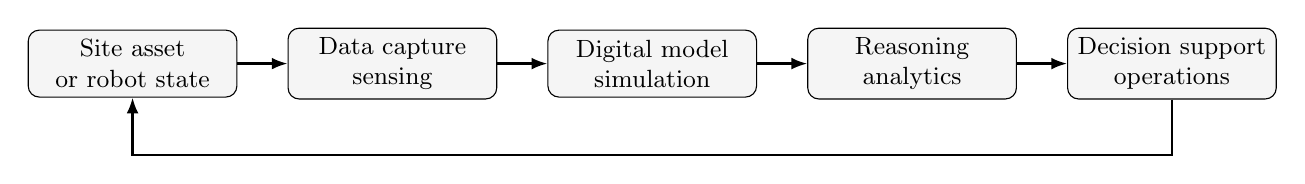
\begin{tikzpicture}[
    box/.style={draw, rounded corners, align=center, minimum height=0.85cm, minimum width=2.65cm, font=\small, fill=gray!8},
    arrow/.style={-{Latex[length=2mm]}, thick}
  ]
    \node[box] (site) at (0,0) {Site asset\\or robot state};
    \node[box] (capture) at (3.3,0) {Data capture\\sensing};
    \node[box] (model) at (6.6,0) {Digital model\\simulation};
    \node[box] (reason) at (9.9,0) {Reasoning\\analytics};
    \node[box] (decision) at (13.2,0) {Decision support\\operations};

    \draw[arrow] (site) -- (capture);
    \draw[arrow] (capture) -- (model);
    \draw[arrow] (model) -- (reason);
    \draw[arrow] (reason) -- (decision);
    \draw[arrow] (decision.south) -- ++(0,-0.7) -| (site.south);
  \end{tikzpicture}}
  \caption{Digital twin literature commonly frames the twin as a closed loop from asset state and sensing to model-based reasoning and operational decisions; the structure is synthesized from \citet{boje2020semantic}, \citet{jiang2021digital}, and \citet{madubuike2022review}.}
  \label{fig:dt-literature}
\end{figure}

\subsection{Construction robotics and inspection}

Construction automation has long promised productivity and safety gains, but adoption is slowed by project-specific site conditions. \citet{bock2015future} describes construction robotics as a field moving toward broader application while still facing technical and organizational limits. \citet{delgado2019robotics} classify robotics and automated systems in construction and highlight adoption challenges such as cost, training, site variability, and unclear integration with existing workflows. These points explain why a small inspection robot twin is a reasonable course project: it tests integration and supervision before attempting physical deployment.

Mobile robots are particularly relevant for progress monitoring and inspection. \citet{asadi2018vision} present a vision-based mobile robotic system for real-time construction applications and emphasize the need for autonomous navigation, sensing, mapping, and real-time processing. Their work is more advanced than this prototype, but the system requirements are similar. A construction inspection robot needs to navigate, observe, and report. It also needs an operator interface because construction engineers are unlikely to interact only through terminal commands.

\begin{figure}[htbp]
  \centering
  \resizebox{0.78\linewidth}{!}{
  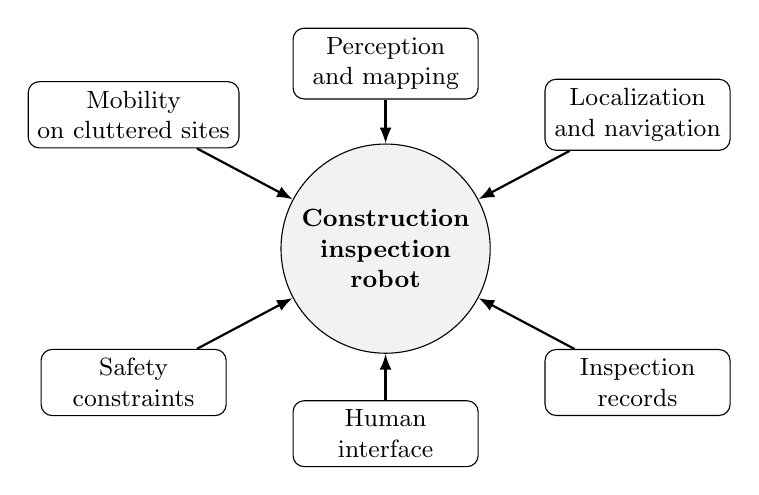
\begin{tikzpicture}[
    core/.style={draw, circle, align=center, minimum size=2.15cm, font=\small\bfseries, fill=gray!10},
    req/.style={draw, rounded corners, align=center, minimum width=2.35cm, minimum height=0.75cm, font=\small, fill=white},
    arrow/.style={-{Latex[length=2mm]}, thick}
  ]
    \node[core] (robot) at (0,0) {Construction\\inspection\\robot};
    \node[req] (mobility) at (-3.2,1.7) {Mobility\\on cluttered sites};
    \node[req] (perception) at (0,2.35) {Perception\\and mapping};
    \node[req] (localization) at (3.2,1.7) {Localization\\and navigation};
    \node[req] (safety) at (-3.2,-1.7) {Safety\\constraints};
    \node[req] (interface) at (0,-2.35) {Human\\interface};
    \node[req] (records) at (3.2,-1.7) {Inspection\\records};

    \foreach \n in {mobility,perception,localization,safety,interface,records}
      \draw[arrow] (\n) -- (robot);
  \end{tikzpicture}}
  \caption{Construction-robotics studies identify recurring requirements around mobility, perception, navigation, safety, interfaces, and data records; the diagram summarizes themes reviewed by \citet{delgado2019robotics} and \citet{asadi2018vision}.}
  \label{fig:robotics-literature}
\end{figure}

Location and tracking research also supports this direction. \citet{teizer2008ultrawideband} discuss real-time location sensing for workforce, equipment, and materials, connecting tracking to construction logistics and safety decisions. The present project uses simulated odometry, LiDAR, and map-frame transforms rather than UWB, but the same decision principle applies: robot position and environment state only become useful when they are made observable and actionable.

\subsection{Navigation, SLAM, and open robot software}

ROS was introduced as an open-source robot software framework to support modular robot development and reuse \citep{quigley2009ros}. ROS 2 continues that idea with a communication layer suitable for distributed nodes, actions, transforms, sensors, and lifecycle-managed systems \citep{ros2humble}. This is why the project separates robot description, navigation, mission orchestration, telemetry, and web bridge responsibilities instead of writing one monolithic script.

For autonomous mobile robots, navigation is the operational core. The Nav2 stack provides localization, planning, control, costmaps, behavior trees, and recovery behaviours for ROS 2 robots \citep{macenski2020marathon, nav2humble}. This project uses Nav2's \texttt{NavigateToPose} action and costmap pipeline rather than writing a custom path planner. That design choice is appropriate for a digital twin prototype because the research question is system integration in a construction context, not low-level planner invention.

SLAM is also relevant because construction layouts change. \citet{kohlbrecher2011slam} present a flexible SLAM system that supports mapping from laser scans. In this implementation, SLAM Toolbox is included in a separate mapping launch workflow. The saved map is then loaded by Nav2 for normal navigation. This separation mirrors a practical construction workflow: map the environment, save a usable representation, then run inspection missions against that representation.

\subsection{Human supervision and telemetry}

Construction robotics should not be treated as full autonomy without supervision. The site engineer needs to know whether the robot is waiting, navigating, blocked, or finished. The digital twin therefore needs a telemetry layer. In this project, telemetry is not only a visual dashboard; it is a structured JSON payload containing pose, velocity, command velocity, nearest obstacle, gimbal joints, safety warnings, target metadata, and mission events. This makes the system closer to an engineering decision-support tool than a simple simulation.

The literature also points toward semantic and context-aware navigation. \citet{karimi2021semantic} propose using building information to support safer and more meaningful robot navigation on construction sites. This project does not yet connect BIM or IFC data, but the waypoint file and marker node are a small step in that direction: the robot does not navigate to arbitrary coordinates only; it navigates to named inspection points and target metadata that can be displayed to the operator.

\section{Methodology}

\subsection{System architecture}

The code was reviewed by reading the ROS packages, launch files, configuration files, mission nodes, web backend, and frontend dashboard. The implementation is organized into five main subsystems. The robot description package defines the URDF/Xacro robot, collisions, inertias, sensors, and gimbal controllers. The simulation package launches Gazebo and the indoor construction-like world, following the same ROS 2/Gazebo integration pattern described in the official simulation documentation \citep{ros2gazebo}. The navigation package contains Nav2 parameters, the static map, SLAM configuration, RViz configuration, and waypoint definitions. The mission package implements readiness checks, autonomous goal dispatch, manual control, telemetry, video recording support, and RViz markers. The web folder implements the FastAPI bridge and dashboard.

Figure~\ref{fig:architecture} uses the same architecture diagram as the project presentation. The architecture is intentionally bidirectional at the operator layer: the dashboard displays telemetry, but it also sends commands back to the mission and manual control topics.

\begin{figure}[htbp]
  \centering
  \resizebox{\linewidth}{!}{
  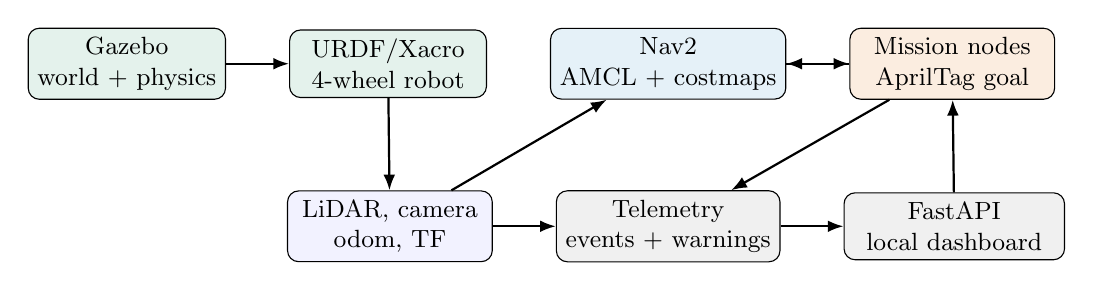
\begin{tikzpicture}[
    node distance=0.6cm and 0.8cm,
    box/.style={draw,rounded corners,align=center,minimum height=0.85cm,font=\small},
    arrow/.style={-{Latex[length=2mm]},thick}
  ]
    \node[box,fill=sitegreen!12,minimum width=2.4cm] (world) {Gazebo\\world + physics};
    \node[box,fill=sitegreen!12,right=of world,minimum width=2.5cm] (robot) {URDF/Xacro\\4-wheel robot};
    \node[box,fill=siteblue!10,right=of robot,minimum width=2.4cm] (nav2) {Nav2\\AMCL + costmaps};
    \node[box,fill=siteorange!14,right=of nav2,minimum width=2.6cm] (mission) {Mission nodes\\AprilTag goal};
    \node[box,fill=gray!12,below=1.15cm of nav2,minimum width=2.8cm] (telemetry) {Telemetry\\events + warnings};
    \node[box,fill=gray!12,right=of telemetry,minimum width=2.8cm] (web) {FastAPI\\local dashboard};
    \node[box,fill=blue!5,left=of telemetry,minimum width=2.6cm] (sensors) {LiDAR, camera\\odom, TF};

    \draw[arrow] (world) -- (robot);
    \draw[arrow] (robot) -- (sensors);
    \draw[arrow] (sensors) -- (nav2);
    \draw[arrow] (nav2) -- (mission);
    \draw[arrow] (mission) -- (nav2);
    \draw[arrow] (mission) -- (telemetry);
    \draw[arrow] (sensors) -- (telemetry);
    \draw[arrow] (telemetry) -- (web);
    \draw[arrow] (web) -- (mission);
  \end{tikzpicture}}
  \caption{Digital twin architecture linking simulation, navigation, mission logic, telemetry, and operator interface.}
  \label{fig:architecture}
\end{figure}

\subsection{Robot, site, and sensing model}

The robot is a compact four-wheel mobile inspection platform. The rear wheels are driven by a Gazebo differential-drive plugin and publish odometry. The model includes collision geometry and inertial values for the chassis, wheels, mast, camera mount, LiDAR, and camera. A pan/tilt camera gimbal is controlled through a ROS 2 control position controller. The robot publishes a LiDAR scan on \texttt{/scan}, camera images on \texttt{/camera/image\_raw}, odometry on \texttt{/odom}, and transforms through the standard TF tree.

The URDF source was checked in \path{src/my_robot_description/urdf/robot.urdf.xacro}. It appears to be a custom course-project model built from primitive URDF geometry rather than a downloaded mesh-based robot. The file defines the \texttt{orbit\_camera\_bot} base, four wheel links, mast, pan/tilt camera joints, LiDAR frame, camera frame, Gazebo material settings, and ROS 2 control interfaces. The model is intentionally simple: the rear wheels are actuated through the Gazebo differential-drive plugin, while the front wheels support the chassis. This is sufficient for the inspection-navigation objective without claiming mobile manipulation.

The Gazebo world represents a small site-like interior rather than an empty laboratory. It includes walls, collision obstacles, construction barriers, material-like blocks, a rebar-style object, a tool chest, an inspection column, and a wall-mounted AprilTag. These details matter because Nav2 costmaps and LiDAR scans need obstacles to reason about. The AprilTag is visually present in the world, but the current autonomous completion logic uses known map coordinates from \texttt{waypoints.yaml}.

\subsection{Navigation and mission execution}

The navigation workflow starts with the robot spawned at point A. In the waypoint file, A is defined at $x=-3.8$ m and $y=-3.6$ m, while the target approach point B is defined at $x=-1.5$ m and $y=3.65$ m with a yaw of 1.5708 rad. The wall AprilTag target is stored separately at $x=-1.5$ m, $y=4.93$ m, and $z=1.05$ m with a completion radius of 1.4 m. This distinction is useful: the robot should not collide with the wall or tag surface, so it navigates to an approach pose rather than the tag position itself.

Nav2 is configured with AMCL, a static map, global and local costmaps, obstacle and inflation layers, a DWB local planner, Navfn global planner, velocity smoothing, and lifecycle management. The robot radius is set to 0.31 m. The local costmap uses a 4 m rolling window and a 0.5 m inflation radius, while the global costmap uses a 0.6 m inflation radius. Linear speed is limited to 0.35 m/s and angular speed to 1.2 rad/s. These values are simple but explicit safety constraints.

The mission orchestrator waits for the Nav2 action server and the \texttt{map} to \texttt{base\_link} transform before sending a goal. It publishes compact event strings including readiness, navigation start, acceptance, success, failure status, and AprilTag reached events. To avoid the previous line-overflow issue, the report describes these event names in prose rather than placing a long unbreakable sequence of \texttt{texttt} tokens in one line.

\subsection{Telemetry, markers, and dashboard}

The telemetry node subscribes to mission state, events, odometry, commanded velocity, LiDAR, joint states, orbit status, and video status. It publishes a JSON payload at 5 Hz. The dashboard bridge exposes this payload through HTTP and WebSocket endpoints and converts camera images into a JPEG stream. The frontend displays the mission state, route points, camera stream, manual drive controls, gimbal sliders, pose, velocity, command velocity, nearest obstacle distance, AprilTag metadata, safety warnings, and event log.

RViz is used as the engineering visualization layer. The waypoint marker node publishes waypoint arrows, point labels, target cylinder markers, and AprilTag target markers. The RViz configuration displays the grid, map, robot model, TF, laser scan, mission markers, and camera. This complements the browser dashboard: the dashboard is better for operation, while RViz is better for debugging the robot state in the map frame.

\begin{table}[htbp]
  \centering
  \caption{Implemented modules and evidence found in the project files.}
  \label{tab:modules}
  \begin{tabularx}{\linewidth}{p{0.23\linewidth}X}
    \toprule
    Module & Implemented evidence \\
    \midrule
    Robot description & URDF/Xacro collision geometry, inertias, wheel joints, mast, LiDAR, RGB camera, pan/tilt gimbal, Gazebo plugins, and ROS 2 control joints. \\
    Simulation & Gazebo launch file, indoor room world, construction-like obstacles, inspection column asset, and wall AprilTag target. \\
    Navigation & Nav2 bringup, AMCL initial pose, static map, SLAM Toolbox mapping launch, costmaps, DWB local planner, Navfn planner, velocity smoother, and RViz config. \\
    Mission layer & Start/stop/reset commands, Nav2 readiness check, \texttt{NavigateToPose} dispatch, completion events, waypoint markers, manual drive limits, and gimbal control. \\
    Web twin & FastAPI ROS bridge, WebSocket telemetry stream, HTTP command endpoints, camera stream, dashboard controls, metrics, warnings, and event display. \\
    \bottomrule
  \end{tabularx}
\end{table}

\section{Results and Discussion}

\subsection{Digital twin demonstration}

The prototype completed the intended demonstration workflow: a simulated robot was launched in a construction-like room, localized on a saved map, commanded from a web dashboard, navigated toward the AprilTag approach point, and displayed state through both the dashboard and RViz. Figure~\ref{fig:route-map} shows the corrected 2D site layout, the recorded A--B mission trajectory, and the Gazebo world during the demonstration. Figure~\ref{fig:rviz} adds the RViz frame extracted from the same video, showing the robot, map, scan, TF, and mission markers.

\begin{figure}[htbp]
  \centering
  \begin{subfigure}[t]{0.49\linewidth}
    \centering
    \resizebox{\linewidth}{!}{
    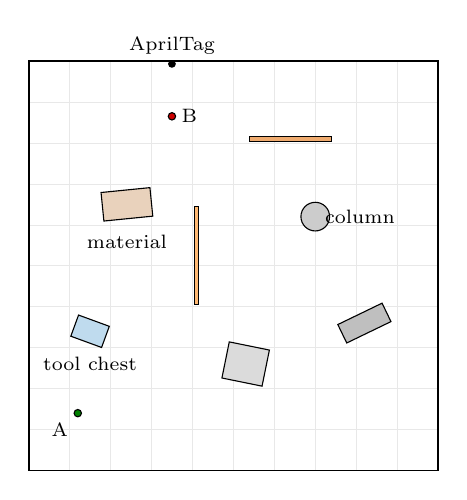
\begin{tikzpicture}[
      x=0.52cm,y=0.52cm,
      wall/.style={draw, line width=0.7pt},
      obs/.style={draw, fill=gray!25},
      barrier/.style={draw, fill=orange!55},
      label/.style={font=\scriptsize}
    ]
      \draw[step=1, gray!18, very thin] (-5,-5) grid (5,5);
      \draw[wall] (-5,-5) rectangle (5,5);
      \begin{scope}[shift={(-2.6,1.5)},rotate=5.7]\draw[obs, fill=brown!35] (-0.6,-0.35) rectangle (0.6,0.35);\end{scope}
      \begin{scope}[shift={(0.3,-2.4)},rotate=-11.5]\draw[obs, fill=gray!28] (-0.5,-0.45) rectangle (0.5,0.45);\end{scope}
      \begin{scope}[shift={(3.2,-1.4)},rotate=25.8]\draw[obs, fill=gray!50] (-0.6,-0.25) rectangle (0.6,0.25);\end{scope}
      \begin{scope}[shift={(-0.9,0.25)},rotate=90]\draw[barrier] (-1.2,-0.04) rectangle (1.2,0.04);\end{scope}
      \begin{scope}[shift={(1.4,3.1)},rotate=0]\draw[barrier, fill=siteorange!65] (-1.0,-0.06) rectangle (1.0,0.06);\end{scope}
      \begin{scope}[shift={(-3.5,-1.6)},rotate=-20.1]\draw[obs, fill=siteblue!25] (-0.4,-0.275) rectangle (0.4,0.275);\end{scope}
      \draw[obs, fill=gray!40] (2.0,1.2) circle (0.35);
      \draw[fill=black] (-1.5,4.93) circle (0.08);
      \node[label, above] at (-1.5,4.93) {AprilTag};
      \draw[fill=green!50!black] (-3.8,-3.6) circle (0.09);
      \node[label, below left] at (-3.8,-3.6) {A};
      \draw[fill=red!80!black] (-1.5,3.65) circle (0.09);
      \node[label, right] at (-1.5,3.65) {B};
      \node[label, below] at (-2.6,1.0) {material};
      \node[label, right] at (2.0,1.2) {column};
      \node[label, below] at (-3.5,-2.0) {tool chest};
    \end{tikzpicture}}
    \caption{Corrected 2D site layout redrawn from \texttt{indoor\_room.world} poses.}
  \end{subfigure}
  \hfill
  \begin{subfigure}[t]{0.49\linewidth}
    \centering
    \resizebox{\linewidth}{!}{
    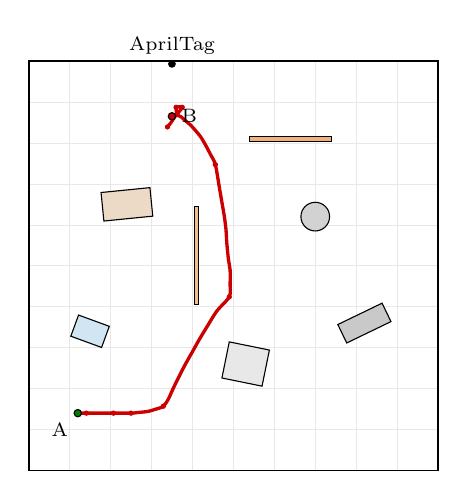
\begin{tikzpicture}[
      x=0.52cm,y=0.52cm,
      wall/.style={draw, line width=0.7pt},
      obs/.style={draw, fill=gray!18},
      path/.style={draw=red!80!black, line width=1.2pt},
      label/.style={font=\scriptsize}
    ]
      \draw[step=1, gray!18, very thin] (-5,-5) grid (5,5);
      \draw[wall] (-5,-5) rectangle (5,5);
      \begin{scope}[shift={(-2.6,1.5)},rotate=5.7]\draw[obs, fill=brown!30] (-0.6,-0.35) rectangle (0.6,0.35);\end{scope}
      \begin{scope}[shift={(0.3,-2.4)},rotate=-11.5]\draw[obs] (-0.5,-0.45) rectangle (0.5,0.45);\end{scope}
      \begin{scope}[shift={(3.2,-1.4)},rotate=25.8]\draw[obs, fill=gray!42] (-0.6,-0.25) rectangle (0.6,0.25);\end{scope}
      \begin{scope}[shift={(-0.9,0.25)},rotate=90]\draw[obs, fill=siteorange!50] (-1.2,-0.04) rectangle (1.2,0.04);\end{scope}
      \begin{scope}[shift={(1.4,3.1)},rotate=0]\draw[obs, fill=siteorange!60] (-1.0,-0.06) rectangle (1.0,0.06);\end{scope}
      \begin{scope}[shift={(-3.5,-1.6)},rotate=-20.1]\draw[obs, fill=siteblue!18] (-0.4,-0.275) rectangle (0.4,0.275);\end{scope}
      \draw[obs, fill=gray!35] (2.0,1.2) circle (0.35);
      \draw[path] plot[smooth] coordinates {
        (-3.80,-3.60) (-3.72,-3.60) (-3.64,-3.60) (-3.59,-3.60)
        (-3.48,-3.60) (-3.36,-3.60) (-3.25,-3.60) (-3.12,-3.60)
        (-3.02,-3.60) (-2.93,-3.60) (-2.82,-3.60) (-2.75,-3.60)
        (-2.68,-3.60) (-2.60,-3.60) (-2.54,-3.60) (-2.50,-3.60)
        (-2.48,-3.60) (-2.46,-3.60) (-2.38,-3.59) (-2.29,-3.58)
        (-2.18,-3.57) (-2.05,-3.55) (-1.92,-3.51) (-1.82,-3.48)
        (-1.71,-3.43) (-1.60,-3.28) (-1.48,-3.02) (-1.35,-2.75)
        (-1.18,-2.42) (-1.00,-2.10) (-0.82,-1.78) (-0.62,-1.45)
        (-0.40,-1.10) (-0.10,-0.76) (-0.08,-0.45) (-0.08,-0.10)
        (-0.12,0.15) (-0.16,0.55) (-0.18,0.88) (-0.22,1.20)
        (-0.28,1.55) (-0.34,1.90) (-0.44,2.47) (-0.56,2.72)
        (-0.68,2.95) (-0.80,3.15) (-0.94,3.32) (-1.06,3.45)
        (-1.18,3.55) (-1.28,3.64) (-1.37,3.69) (-1.40,3.87)
        (-1.33,3.88) (-1.25,3.87) (-1.31,3.78) (-1.43,3.64)
        (-1.52,3.50) (-1.61,3.39)
      };
      \foreach \p in {(-3.59,-3.60),(-2.93,-3.60),(-2.50,-3.60),(-1.71,-3.43),(-0.10,-0.76),(-0.44,2.47),(-1.37,3.69),(-1.40,3.87),(-1.25,3.87),(-1.61,3.39)}
        \fill[red!80!black] \p circle (0.065);
      \draw[fill=green!50!black] (-3.8,-3.6) circle (0.09);
      \node[label, below left] at (-3.8,-3.6) {A};
      \draw[fill=red!80!black] (-1.5,3.65) circle (0.09);
      \node[label, right] at (-1.5,3.65) {B};
      \draw[fill=black] (-1.5,4.93) circle (0.08);
      \node[label, above] at (-1.5,4.93) {AprilTag};
    \end{tikzpicture}}
    \caption{Recorded A--B mission trajectory.}
  \end{subfigure}
  \vspace{0.4em}
  \begin{subfigure}[t]{0.74\linewidth}
    \centering
    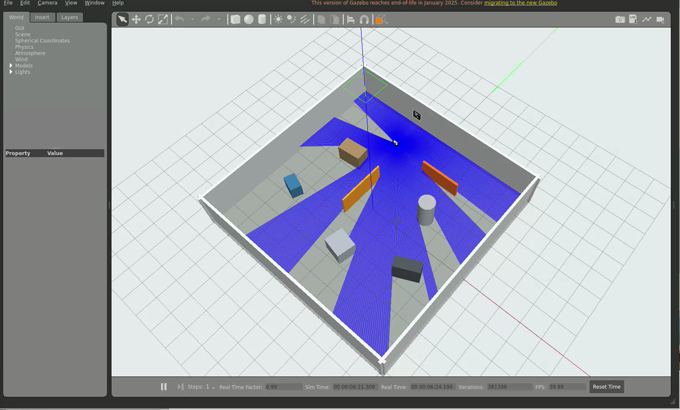
\includegraphics[width=\linewidth]{figures/gazebo_world_snapshot.png}
    \caption{Gazebo world screenshot from the recorded demonstration.}
  \end{subfigure}
  \caption{Navigation evidence used by the digital twin. The 2D obstacles follow the Gazebo world poses, and the trajectory shows the recorded A--B mission path.}
  \label{fig:route-map}
\end{figure}

\begin{figure}[htbp]
  \centering
  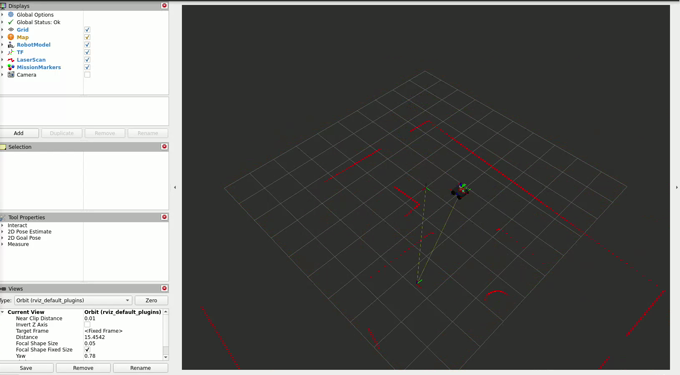
\includegraphics[width=0.82\linewidth]{figures/rviz_snapshot.png}
  \caption{RViz snapshot extracted from the recorded mission video, showing map-frame visualization of the robot, scan, TF, and mission markers.}
  \label{fig:rviz}
\end{figure}

The route is short, but the integration is non-trivial. The system must bring up Gazebo, spawn the URDF robot, publish robot state, activate controllers, run Nav2 lifecycle nodes, publish the initial pose, serve the dashboard, and coordinate the mission command. If any piece is missing, the mission node reports a readiness failure rather than silently sending a goal. This is important for construction use because engineering demonstrations often fail at integration boundaries, not at one isolated algorithm.

\subsection{Operator observability}

The dashboard screenshot in Figure~\ref{fig:web} shows why the web interface is useful. A user can see the mission state, route metadata, camera stream, pose, velocity, nearest obstacle, AprilTag target, safety panel, and event log without reading ROS topics manually. The dashboard does not replace RViz, but it creates an operator-facing view that is closer to what a construction engineer would need during inspection.

\begin{figure}[htbp]
  \centering
  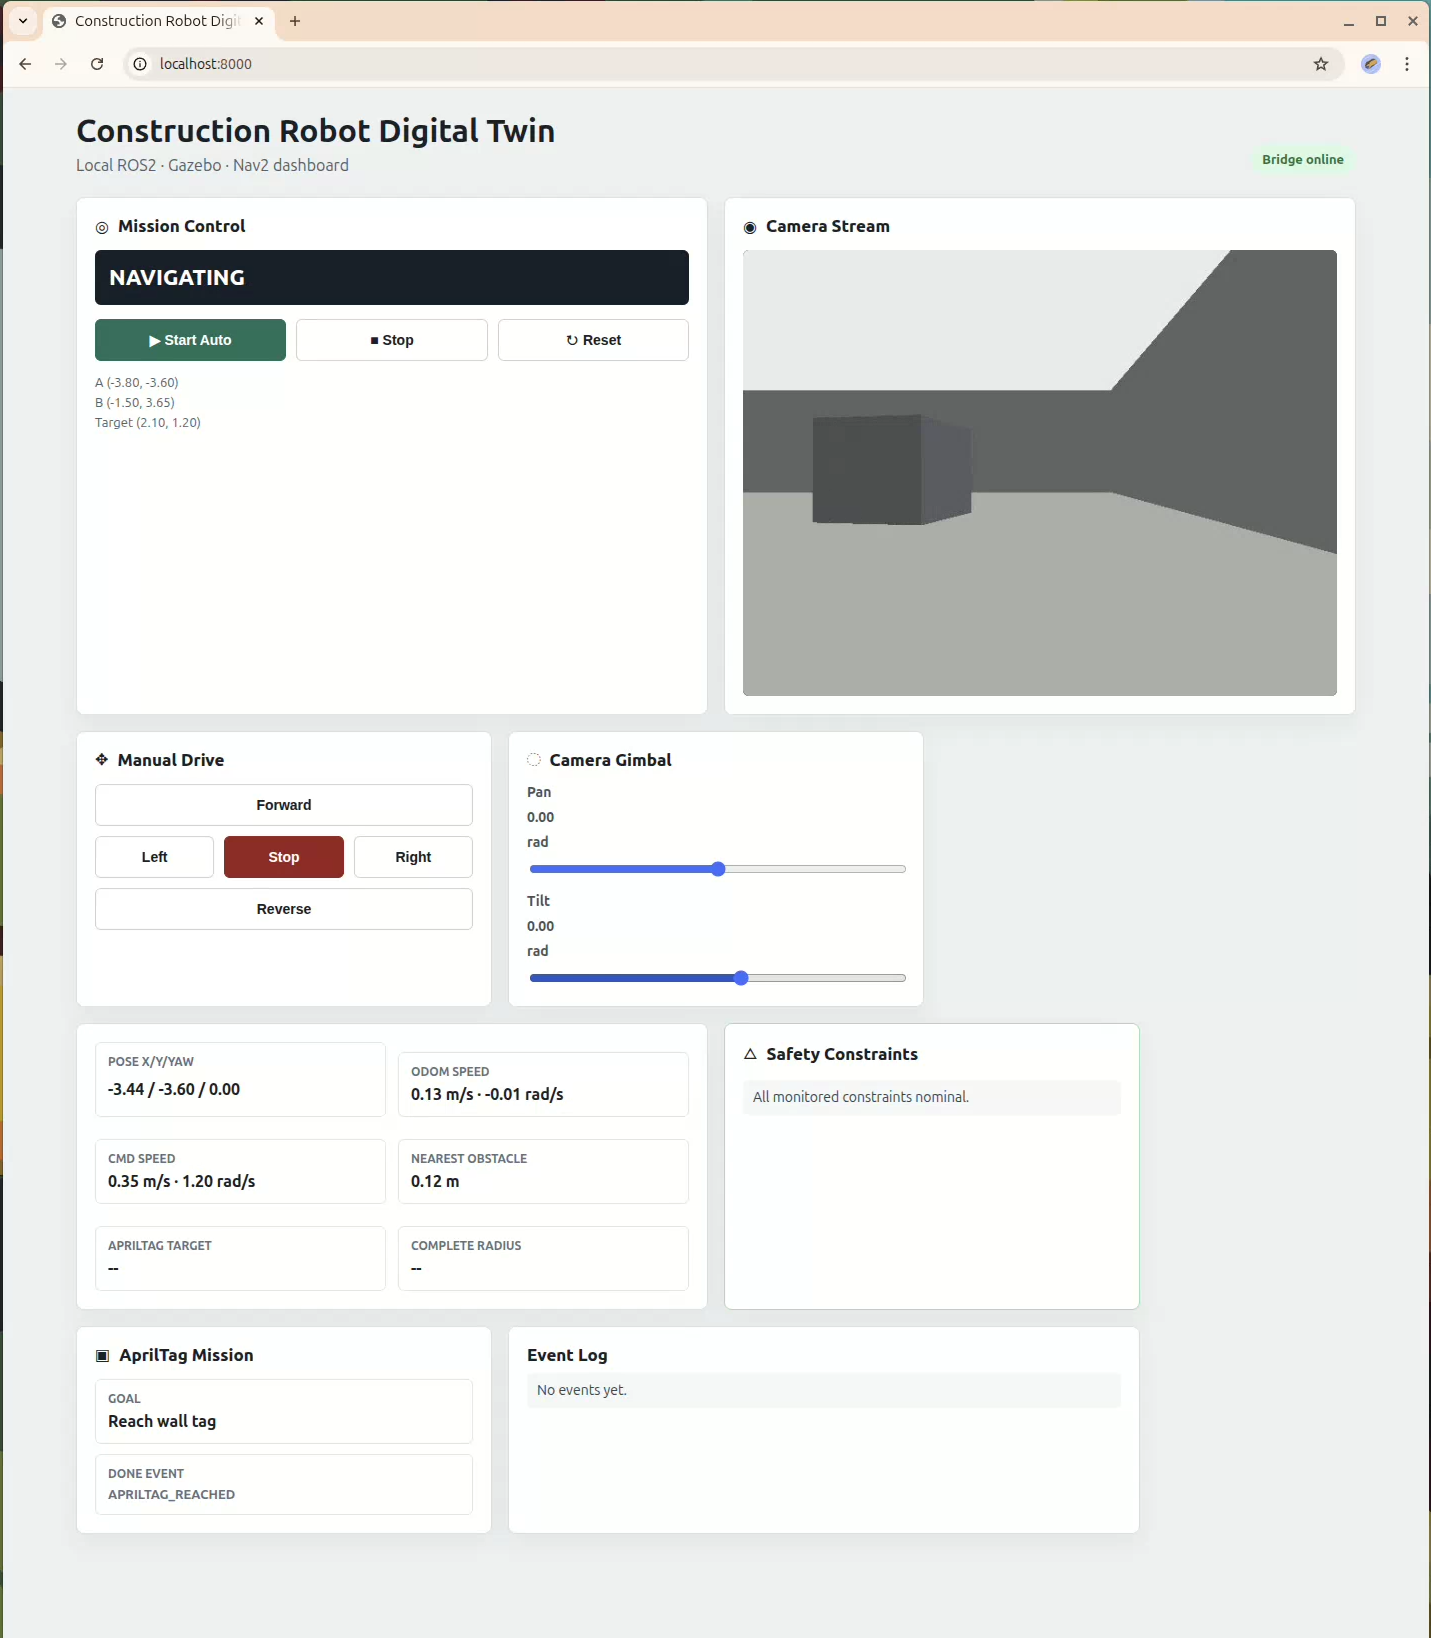
\includegraphics[width=0.9\linewidth]{figures/web.png}
  \caption{Local web dashboard for mission commands, manual control, camera stream, telemetry, warnings, and events.}
  \label{fig:web}
\end{figure}

The telemetry design also creates a path for future data logging. Since the node publishes structured JSON, the same payload could be stored in a time-series database, connected to a project dashboard, or used for post-mission analysis. In the current course prototype, the data are shown live rather than archived, but the interface design is already compatible with a more persistent digital twin workflow.

\subsection{Construction relevance}

The project is relevant to construction because it represents the robot as part of a site operation rather than as a generic indoor robot. The target is a wall-mounted inspection object. The map contains barriers, material-like objects, and a column. Safety is represented through collision geometry, costmap inflation, speed limits, obstacle warnings, and an immediate stop command. These details are small, but they move the prototype toward construction engineering concerns: where the robot can move, what it is inspecting, and what the operator can observe.

At the same time, the prototype should not be interpreted as a deployable site robot. Real construction sites have dust, lighting variation, temporary occlusions, reflective materials, uneven surfaces, people, communication issues, and regulatory constraints. The simulated LiDAR and camera are cleaner than real sensors. The map is known and small. The AprilTag is not detected from images. Therefore, the correct conclusion is that the project demonstrates an architecture and workflow, not field readiness.

\subsection{Limitations and future work}

Four limitations stand out. First, the AprilTag target is not used for visual pose estimation. The mission currently navigates to a known map coordinate and checks proximity to the stored tag position. Second, there is no manipulator arm or MoveIt 2 planning, so the prototype is not a mobile manipulator. Third, the web dashboard does not yet display the costmap or LiDAR scan directly, so RViz remains necessary for debugging. Fourth, the system has not been tested with real robot hardware.

Future work should first close the loop between visual perception and navigation. AprilTag detection could estimate the final tag pose and support a short visual-servoing approach. The dashboard could display a simplified map, scan, and costmap overlay. If the project is later extended into mobile manipulation, MoveIt 2 planning would need to be added with construction obstacles represented as collision objects. Physical deployment would also require calibration, sensor noise handling, emergency stop hardware, and safety procedures for human-robot coexistence.

\section{Conclusions}

This paper presented a ROS 2 construction robot digital twin prototype for mobile inspection. The project integrates Gazebo simulation, a robot model, Nav2 navigation, SLAM-ready mapping, mission logic, telemetry, RViz visualization, and a web dashboard. The system is grounded in construction digital twin literature because it links a virtual site, robot state, mission events, sensor streams, and operator decisions. It is also grounded in construction robotics literature because it focuses on inspection, navigation, sensing, and supervision rather than only visual animation.

The main result is an executable and observable prototype. The robot can be commanded from the dashboard, navigates from point A to the AprilTag approach point B, and reports state through ROS topics, telemetry JSON, RViz markers, and browser UI elements. The main engineering value is the clean separation of packages and the explicit handling of readiness, safety constraints, and telemetry. The main limitation is scope: this is a simulated mobile inspection robot twin, not a field-deployed mobile manipulator. Future work should add real AprilTag detection, richer dashboard map visualization, and physical validation before any stronger claim is made.

\section*{Acknowledgements}

The author acknowledges the CIVIL 8025 teaching team at The University of Hong Kong for the project direction and course context. The implementation builds on open-source ROS 2, Gazebo, Nav2, SLAM Toolbox, FastAPI, and related robotics tools.

\bibliographystyle{apacite}
\bibliography{references}

\end{document}
